\section{Dimensionality reduction}


\newcommand{\motivationplot}[1]{
    \begin{tikzpicture}
        \begin{axis}[
            height=7cm,
            width=7cm,
            xlabel=$x_1$,
            ylabel=$x_2$,
            xmajorticks=false,
            ymajorticks=false
        ]
            \ifnum#1=0
                \addplot[
                    only marks,
                    blue,
                    opacity=0.5
                ] coordinates {
                    (-0.025, -0.056) %0
                    (-0.017, 0.026) %1
                    (-0.061, -0.061) %2
                    (0.01, -0.005) %3
                    (-0.073, -0.022) %4
                    (0.126, 0.126) %5
                    (0.132, 0.1) %6
                    (0.063, 0.121) %7
                    (0.099, 0.165) %8
                    (0.104, 0.079) %9
                    (0.16, -0.11) %10
                    (0.138, -0.157) %11
                    (0.153, -0.081) %12
                    (0.11, -0.1) %13
                    (0.122, -0.114) %14
                };
            \fi
            \ifnum#1=1
                \addplot[
                    only marks,
                    blue,
                    opacity=0.5
                ] (x, x + rand);
            \fi
        \end{axis}
    \end{tikzpicture}
}

\newsavebox{\motivationclusters}
\sbox{\motivationclusters}{
    \motivationplot{0}
}
\newsavebox{\motivationaxes}
\sbox{\motivationaxes}{
    \motivationplot{1}
}

\newsavebox{\overfitting}
\sbox{\overfitting}{
    \begin{tikzpicture}
        \begin{axis}[
            height=6cm,
            width=8cm,
            axis lines=left,
            xmajorticks=false,
            ymajorticks=false,
            ylabel=Loss,
            xlabel=$|p|$,
            ymin=-2,
            xmin=-1,
            xmax=3
        ]
            \addplot[thick, red, domain=-1:3, samples=100] (x, x^2);
        \end{axis}
    \end{tikzpicture}
}

\newcommand{\predictorplot}[3]{
    \nextgroupplot[
        xlabel=\footnotesize{#1},
        ylabel=\footnotesize{#2},
        ytick=#3
    ]
        \addplot[
            only marks,
            blue,
            opacity=0.5
        ] table [
            col sep=comma,
            x=#1,
            y=mpg
        ] {data/scaledauto.csv};
}

\newcommand{\coefplot}[4]{
    \predictorplot{#1}{#2}{#3}
        \addplot[
            red
        ] coordinates {
            (-5, 23.445-5*#4)
            (5, 23.445+5*#4)
        };
}

\newcommand{\correlationplot}[1]{
    \begin{tikzpicture}
        \begin{groupplot}[
            group style={
                group size=3 by 2,
                vertical sep=0.8cm,
                horizontal sep=0.05cm
            },
            height=4cm,
            width=4.6cm,
            ticklabel style={font=\footnotesize},
            xtick pos=bottom,
            ytick pos=left,
            x label style={yshift=0.15cm},
            y label style={yshift=-0.15cm},
            ymin=0,
            ymax=52,
            xmin=-4,
            xmax=4,
            xtick={-3, 0, 3}
        ]
            \ifnum#1=0
                \predictorplot{cylinders}{mpg}{{10, 20, 30, 40, 50}}
                \predictorplot{displacement}{}{\empty}
                \predictorplot{horsepower}{}{\empty}
                \predictorplot{weight}{mpg}{{10, 20, 30, 40, 50}}
                \predictorplot{acceleration}{}{\empty}
                \predictorplot{year}{}{\empty}
            \fi
            \ifnum#1=1
                \coefplot{cylinders}{mpg}{{10, 20, 30, 40, 50}}{-0.561}
                \coefplot{displacement}{}{\empty}{0.802}
                \coefplot{horsepower}{}{\empty}{-0.015}
                \coefplot{weight}{mpg}{{10, 20, 30, 40, 50}}{-5.763}
                \coefplot{acceleration}{}{\empty}{0.234}
                \coefplot{year}{}{\empty}{2.771}
            \fi
        \end{groupplot}
    \end{tikzpicture}
}

\newsavebox{\correlationpredictors}
\sbox{\correlationpredictors}{
    \correlationplot{0}
}
\newsavebox{\correlationcoefs}
\sbox{\correlationcoefs}{
    \correlationplot{1}
}

\newsavebox{\heatmap}
\sbox{\heatmap}{
    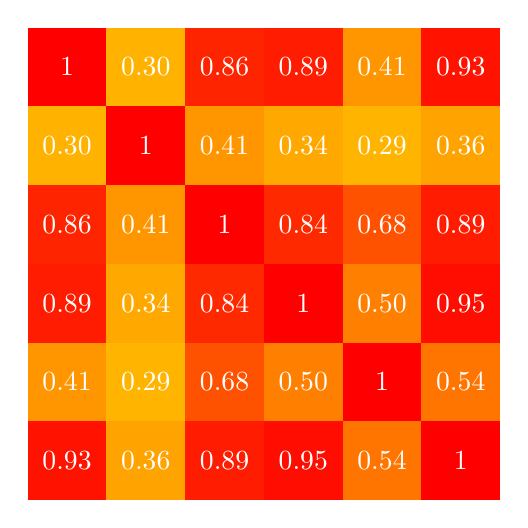
\begin{tikzpicture}
        \foreach \y [count=\n] in {
            {1,0.30,0.86,0.89,0.41,0.93},
            {0.30,1,0.41,0.34,0.29,0.36},
            {0.86,0.41,1,0.84,0.68,0.89},
            {0.89,0.34,0.84,1,0.50,0.95},
            {0.41,0.29,0.68,0.50,1,0.54},
            {0.93,0.36,0.89,0.95,0.54,1},
          } {
            \foreach \x [count=\m] in \y {
                \pgfmathsetmacro{\colorfraction}{100*\x} % Multiply by 100
              \node[fill=red!\colorfraction!yellow, minimum size=1cm, text=white, inner sep=0pt, outer sep=0pt] at (\m,-\n) {\x};
            }
          }

      \end{tikzpicture}
}

\begin{frame}{Dimensionality reduction: Motivation}
    \begin{tikzpicture}
        \node[] at (-5.25, 3.5) {};
        \node[] at (-5.25, -3.5) {};

        \visible<1>{
            \node[] at (0, 0) {
                \usebox{\motivationclusters}
            };
        }
        \visible<2>{
            \node[] at (0, 0) {
                \usebox{\motivationaxes}
            };
        }
        \visible<3>{
            \node[draw=black, inner sep=0pt, anchor=west] (test) at (-4, 0) {
                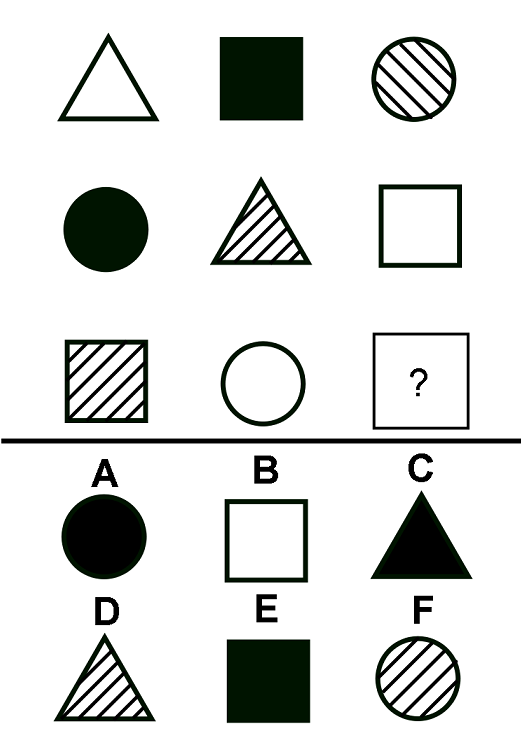
\includegraphics[height=4cm]{data/iqtest.png}
            };
            \node[draw=black, dashed, anchor=east, align=center] (iq) at (4, 0) {
                Intelligence\\quotient
            };
            \draw[-stealth, line width=5pt, gray] (test) -- (iq);
        }
        \visible<4>{
            \node[] at (0, 0) {
                \usebox{\overfitting}
            };
        }
        \visible<5>{
            \node[] at (0, 0) {
                \usebox{\correlationpredictors}
            };
        }
        \visible<6>{
            \node[] at (0, 0) {
                \usebox{\correlationcoefs}
            };
        }
        \visible<7-8>{
            \node[] (heatmap) at (0, 0) {
                \usebox{\heatmap}
            };
        }
        \visible<8>{
            \node[minimum size=1cm, draw=black, line width=2pt] at ($ (heatmap.north) + (0.5, -2.62) $) {};
        }
    \end{tikzpicture}
\end{frame}


\newcommand{\pcaplot}[1]{
    \begin{tikzpicture}
        \begin{axis}[
            height=6.5cm,
            width=6.5cm,
            xlabel=$z_\mathrm{weight}$,
            ylabel=$z_\mathrm{horsepower}$,
            xmin=-2,
            xmax=3.5,
            ymin=-2,
            ymax=3
        ]
            \addplot[
                only marks,
                mark=*,
                color=blue,
                opacity=0.1
            ] table [col sep=comma, x=x, y=y] {data/pca_components.csv};

            \ifnum#1>0
                \addplot[only marks, mark=*, color=red] coordinates {
                    (-1.81260902e-16, -1.81260902e-17)
                };
            \fi

            \ifnum#1=2
                \draw[red,-stealth,very thick] (axis cs: -1.81260902e-16, -1.81260902e-17) -- (axis cs: -1.81260902e-16 + 0.96677463, -1.81260902e-17 + 0.96677463);
                \node[anchor=north, outer sep=3pt] at (axis cs: -1.81260902e-16 + 0.5 * 0.96677463, -1.81260902e-17 + 0.5 * 0.96677463) {\Large{\textbf{\textcolor{red}{$v$}}}};
            \fi

            \ifnum#1>2
                \draw[red,-stealth,very thick] (axis cs: -1.81260902e-16 - 5 * 0.96677463, -1.81260902e-17 - 5 * 0.96677463) -- (axis cs: -1.81260902e-16 + 5 * 0.96677463, -1.81260902e-17 + 5 * 0.96677463);
                \draw[red,|-|,very thick] (axis cs: -1.81260902e-16 - 1 * 0.96677463, -1.81260902e-17 - 1 * 0.96677463) -- (axis cs: -1.81260902e-16 + 1 * 0.96677463, -1.81260902e-17 + 1 * 0.96677463);
                \draw[red,|-|,very thick] (axis cs: -1.81260902e-16 - 2 * 0.96677463, -1.81260902e-17 - 2 * 0.96677463) -- (axis cs: -1.81260902e-16 + 2 * 0.96677463, -1.81260902e-17 + 2 * 0.96677463);

                \node[rotate=45, anchor=north, inner sep=5pt] at (axis cs: -1.81260902e-16 - 1 * 0.96677463, -1.81260902e-17 - 1 * 0.96677463) {\Large{\textbf{\textcolor{red}{-1}}}};
                \node[rotate=45, anchor=north, inner sep=5pt] at (axis cs: -1.81260902e-16 - 2 * 0.96677463, -1.81260902e-17 - 2 * 0.96677463) {\Large{\textbf{\textcolor{red}{-2}}}};
                \node[rotate=45, anchor=north, inner sep=5pt] at (axis cs: -1.81260902e-16 + 1 * 0.96677463, -1.81260902e-17 + 1 * 0.96677463) {\Large{\textbf{\textcolor{red}{1}}}};
                \node[rotate=45, anchor=north, inner sep=5pt] at (axis cs: -1.81260902e-16 + 2 * 0.96677463, -1.81260902e-17 + 2 * 0.96677463) {\Large{\textbf{\textcolor{red}{2}}}};
                \node[rotate=45, anchor=south, inner sep=3pt] at (axis cs: -1.81260902e-16 + 2.5 * 0.96677463, -1.81260902e-17 + 2.5 * 0.96677463) {\Large{\textbf{\textcolor{red}{$PC_1$}}}};
            \fi

            \ifnum#1=4
                \draw[red,-stealth,very thick] (axis cs: -1.81260902e-16, -1.81260902e-17) -- (axis cs: -1.81260902e-16 + 3 * 0.26058464, -1.81260902e-17 - 3 * 0.26058464);
                \node[anchor=west, outer sep=3pt] at (axis cs: -1.81260902e-16 + 0.8 * 0.26058464, -1.81260902e-17 - 0.8 * 0.26058464) {\Large{\textbf{\textcolor{red}{$v$}}}};
            \fi
        \end{axis}
    \end{tikzpicture}
}

\newsavebox{\pcavariables}
\sbox{\pcavariables}{
    \pcaplot{0}
}
\newsavebox{\pcacenter}
\sbox{\pcacenter}{
    \pcaplot{1}
}
\newsavebox{\pcavector}
\sbox{\pcavector}{
    \pcaplot{2}
}
\newsavebox{\pcafirst}
\sbox{\pcafirst}{
    \pcaplot{3}
}
\newsavebox{\pcasecondvector}
\sbox{\pcasecondvector}{
    \pcaplot{4}
}

\begin{frame}{Dimensionality reduction: Principal component analysis}
    \begin{tikzpicture}
        \node[] at (-5.25, 3.5) {};
        \node[] at (-5.25, -3.5) {};

        \visible<1>{
            \node[] at (0, 0.5) {
                \usebox{\pcavariables}
            };
        }
        \visible<2>{
            \node[] at (0, 0.5) {
                \usebox{\pcacenter}
            };
            \node[] at (0, -3) {
                $c \rightarrow$ center of the data
            };
        }
        \visible<3>{
            \node[] at (0, 0.5) {
                \usebox{\pcavector}
            };
            \node[] at (0, -3) {
                $v \rightarrow$ direction of maximum variance
            };
        }
        \visible<4>{
            \node[] at (0, 0.5) {
                \usebox{\pcafirst}
            };
            \node[] at (0, -3) {
                $PC_1 \rightarrow 0.69*z_\mathrm{horsepower}+0.71*z_\mathrm{weight}$
            };
        }
        \visible<5>{
            \node[] at (0, 0.5) {
                \usebox{\pcasecondvector}
            };
            \node[] at (0, -3) {
                $v \rightarrow$ direction of maximum variance \textbf{orthogonal} to $PC_1$
            };
        }
    \end{tikzpicture}
\end{frame}
